\documentclass[12pt,a4paper]{article}
\usepackage[utf8]{inputenc}
\usepackage{graphicx}
\usepackage{float}
\usepackage{hyperref}
\usepackage{booktabs}
\usepackage[margin=1in]{geometry}
\usepackage{tabularx}
\usepackage{caption}

\title{\textbf{Semantic-Adaptive Hilbert (SAH) Indexing System}\\
\large Code-Aligned Comprehensive Design Document}
\author{}
\date{}

\begin{document}
\maketitle

\section{Executive Summary}
The Semantic-Adaptive Hilbert (SAH) Indexing System is a specialized spatial data processing pipeline. Unlike standard quadtrees that blindly subdivide space, SAH utilizes \textbf{Coastline-aware Adaptive Quadtree Segmentation} to construct an initial asymmetric grid, followed by \textbf{Local Adaptive Hilbert Indexing} to serialize the spatial data. This decoupled approach minimizes empty data processing, reduces memory footprints, and guarantees $O(\log B + \log N + K)$ query speeds via R-Tree and Local Hilbert Bisection caching mechanisms.

\section{System Architecture \& Flow}
The system is organized into a linear pre-processing pipeline followed by an optimized in-memory query engine.

\begin{figure}[H]
    \centering
    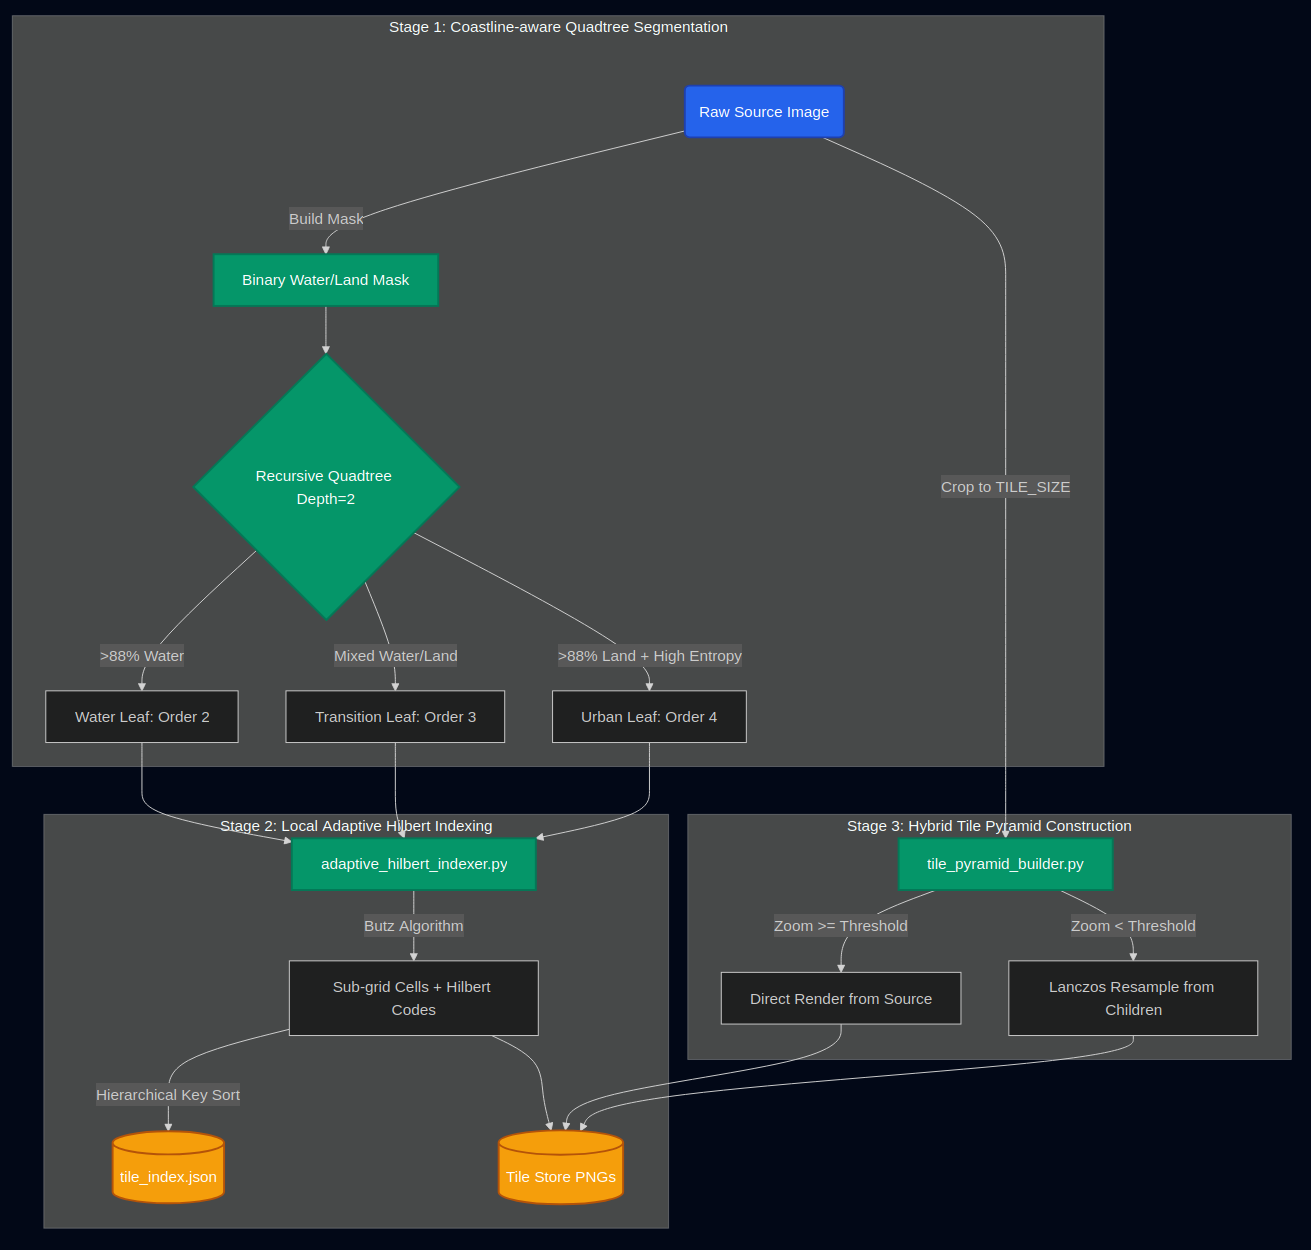
\includegraphics[width=\textwidth]{images/flow.png}
    \caption{System Architecture Flow (Part 1)}
\end{figure}

\begin{figure}[H]
    \centering
    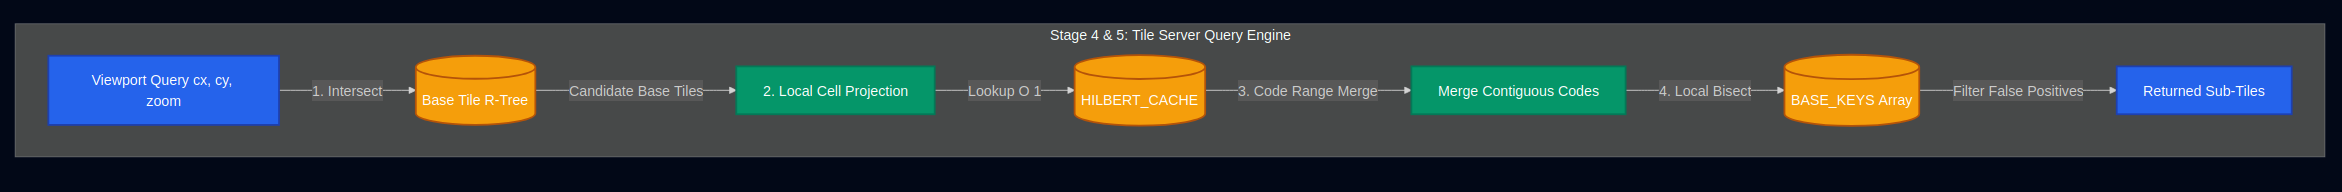
\includegraphics[width=\textwidth]{images/flow_2.png}
    \caption{System Architecture Flow (Part 2)}
\end{figure}

\section{Core Codebase Components}
The SAH Indexing System is driven by a suite of specialized Python and React components that govern ingestion, indexing, and serving.

\begin{itemize}
    \item \textbf{\texttt{region\_segmenter.py}}: Ingestion script. Generates the initial boolean water mask and recursively builds the spatial quadtree. It assigns the semantic class (Water, Transition, Urban) and the baseline Hilbert Order to each leaf node.
    \item \textbf{\texttt{adaptive\_hilbert\_indexer.py}}: Processing script. Takes the quadtree leaves, calculates local Hilbert trajectories using the Butz algorithm, and generates the hierarchically sortable composite keys. Responsible for exporting \texttt{tile\_index.json} and the sub-tile PNG store.
    \item \textbf{\texttt{tile\_pyramid\_builder.py}}: Rendering script. Constructs the adaptive multi-level pyramid (LOD). Crops source boundaries to exact \texttt{TILE\_SIZE} multiples to prevent black stripes, utilizing direct source-rendering for high zooms and Lanczos-resampled $2\times2$ block merging for overview zooms.
    \item \textbf{\texttt{tile\_server.py}}: Backend API \& Query Engine. A Flask server that ingests \texttt{tile\_index.json} into fast RAM structures (\texttt{INDEX}, \texttt{BASE\_KEYS}, \texttt{HILBERT\_CACHE}, \texttt{base\_rtree}) and implements the ultra-fast \texttt{\_hilbert\_range\_scan} endpoint.
    \item \textbf{\texttt{run\_pipeline.py}}: Execution orchestrator. Automates the pipeline, passing the raw gigapixel array sequentially through the segmenter, indexer, and pyramid builder.
    \item \textbf{\texttt{HilbertViewer.jsx}}: Frontend interface. A React-based interactive canvas that communicates with the Flask API. Dynamically calculates and renders the cosmetic Display Render Order for contextual spatial UI scaling.
\end{itemize}

\section{Pipeline Stages \& Code Execution Flow}

\subsection{Stage 1: Coastline-aware Quadtree Segmentation}
Instead of a rigid grid, the image is decomposed via a recursive quadtree bounded to a maximum depth of 2.

\paragraph{Step A: Binary Mask Generation}
A pixel-level mask is generated to cleanly isolate aquatic regions. A pixel is classified as water if the raw channel ratio $(B - R) / (R+G+B) \geq 0.04$.

\paragraph{Step B \& C: Quadtree Subdivision}
Each base tile evaluates its geographic composition against the boolean mask:
\begin{enumerate}
    \item \textbf{Predominantly Water} (water\_fraction $\geq 0.88$): Becomes a \textbf{Water Leaf (Class 0, Hilbert Order 2)} at any depth.
    \item \textbf{Mixed Tile} (water\_fraction between 0.12 and 0.88): Automatically classified as a coastline boundary. Becomes a \textbf{Transition Leaf (Class 1, Order 3)}.
    \item \textbf{Predominantly Land} (water\_fraction $< 0.12$): 
    \begin{itemize}
        \item \textbf{Depth 0:} Automatically split.
        \item \textbf{Depth 1:} Entropy is evaluated. If entropy $\geq 2.80$ and the tile is large enough, it splits again. Otherwise, it defaults to a Transition Leaf.
        \item \textbf{Depth 2:} Reaches maximum depth and becomes an \textbf{Urban Leaf (Class 2, Order 4)}.
    \end{itemize}
\end{enumerate}

\begin{figure}[H]
    \centering
    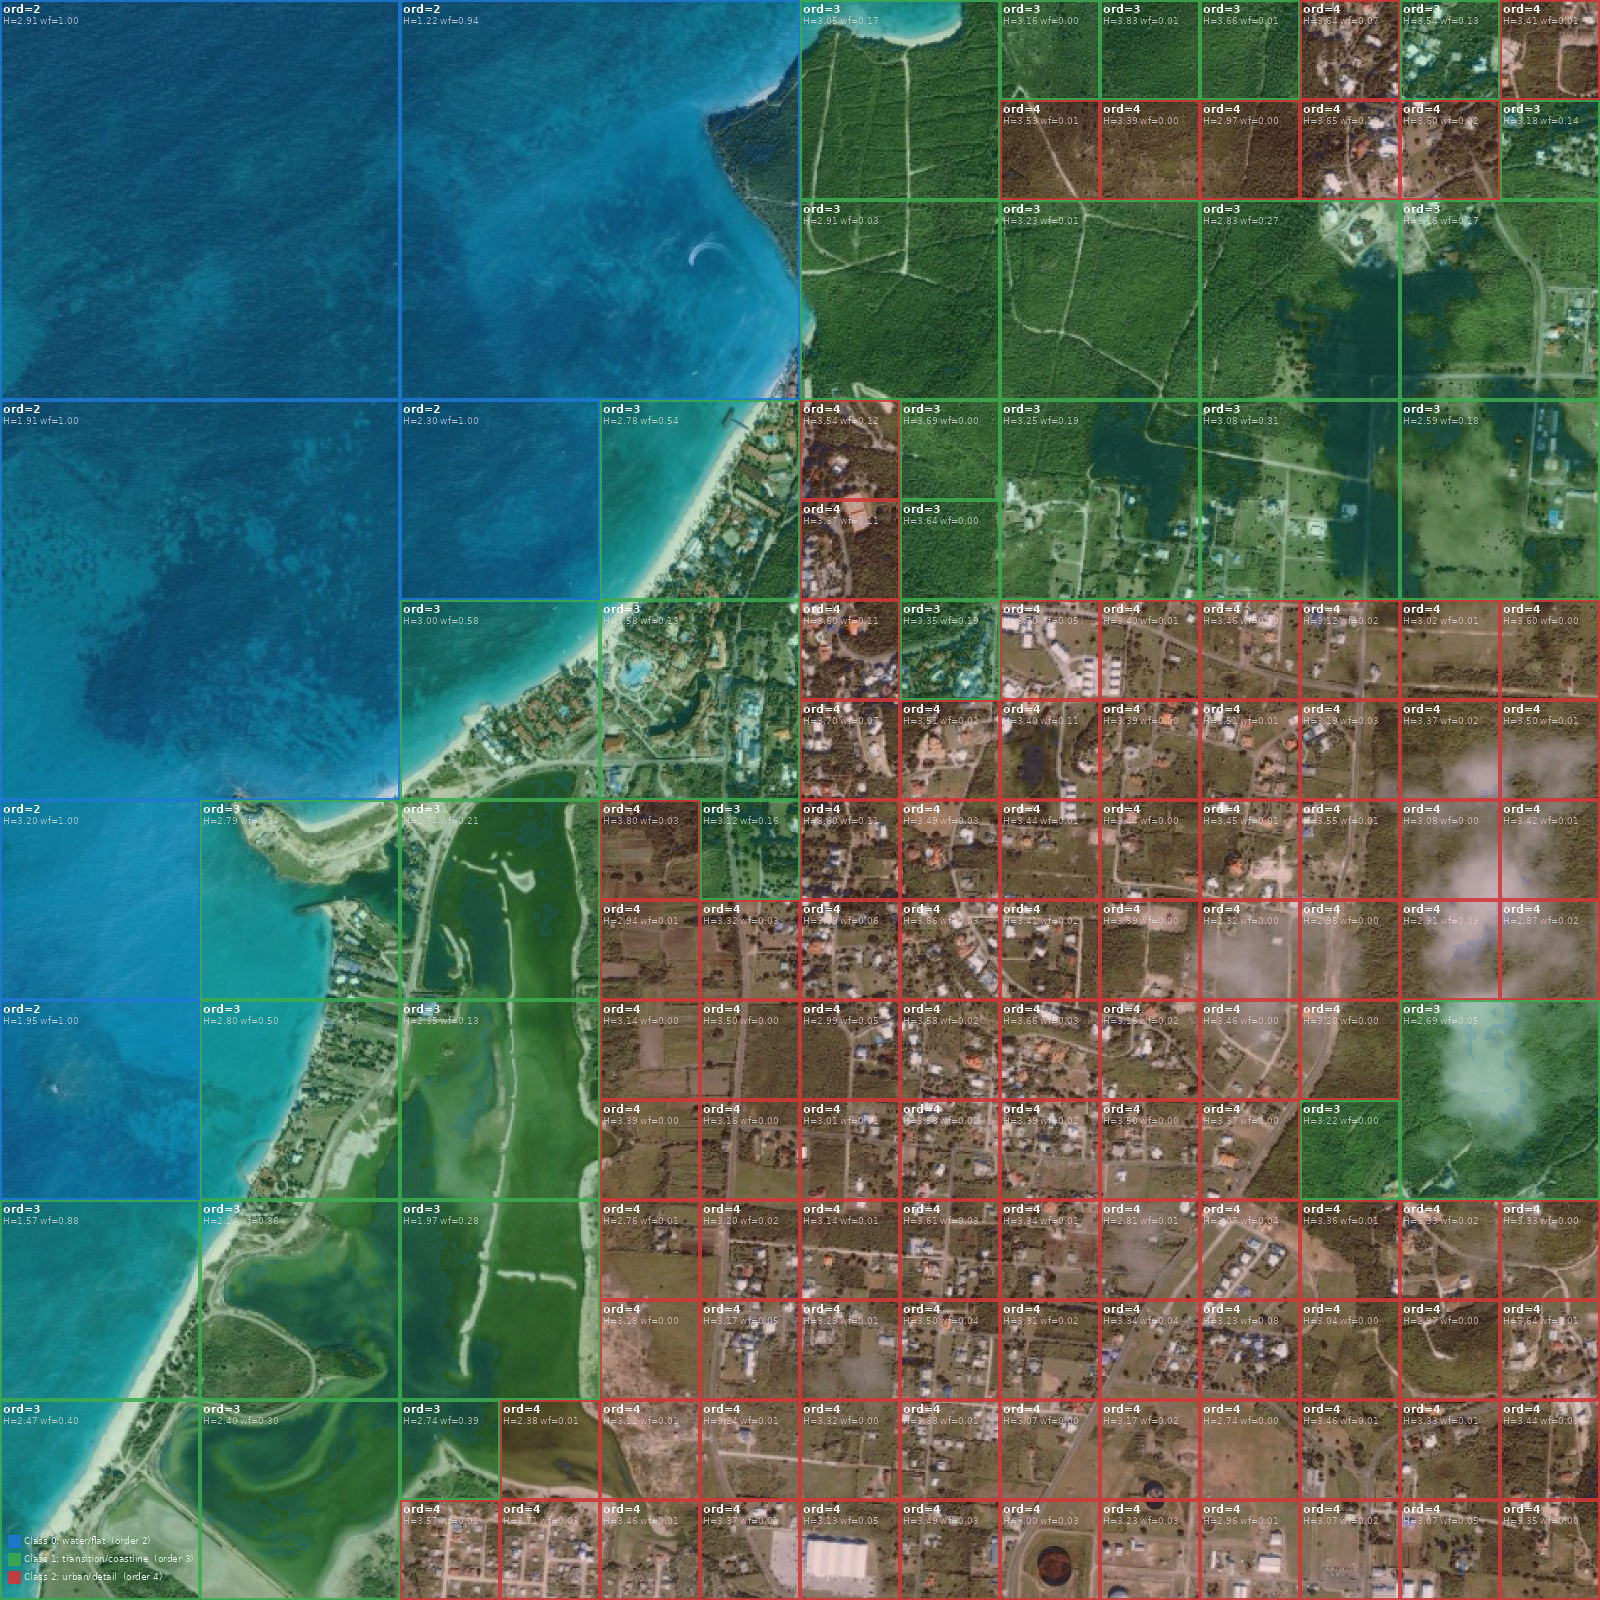
\includegraphics[width=0.8\textwidth]{images/segmentation_vis.png}
    \caption{The output of region\_segmenter.py, detailing the asymmetric quadtree and specific regional classes.}
\end{figure}

\subsection{Stage 2: Local Adaptive Hilbert Indexing}
Each resulting quadtree leaf is subdivided into an adaptive sub-grid based on its Hilbert Order (Order 2 $\rightarrow$ $4\times4$ grid, Order 3 $\rightarrow$ $8\times8$ grid, Order 4 $\rightarrow$ $16\times16$ grid).

\begin{enumerate}
    \item \textbf{Subdivision \& Hilbert Coding:} For each sub-cell, a Hilbert code is mathematically calculated using the Butz algorithm.
    \item \textbf{Key Generation:} A sortable hierarchical composite string key is generated for every sub-cell: \\
    \texttt{\{class\}\_\{order\}\_\{base\_tx\}\{base\_ty\}\_\{sub\_x\}\{sub\_y\}\_\{hilbert\}}
    \item \textbf{Data Localization:} Sub-cells are saved as PNG tiles, and their metadata is written to \texttt{tile\_index.json}. Crucially, because the composite key begins with \texttt{base\_tx} and \texttt{base\_ty}, \textbf{the indexing is localized to the quadtree base tile}, allowing for isolated, parallelizable binary searches during queries.
\end{enumerate}

\begin{figure}[H]
    \centering
    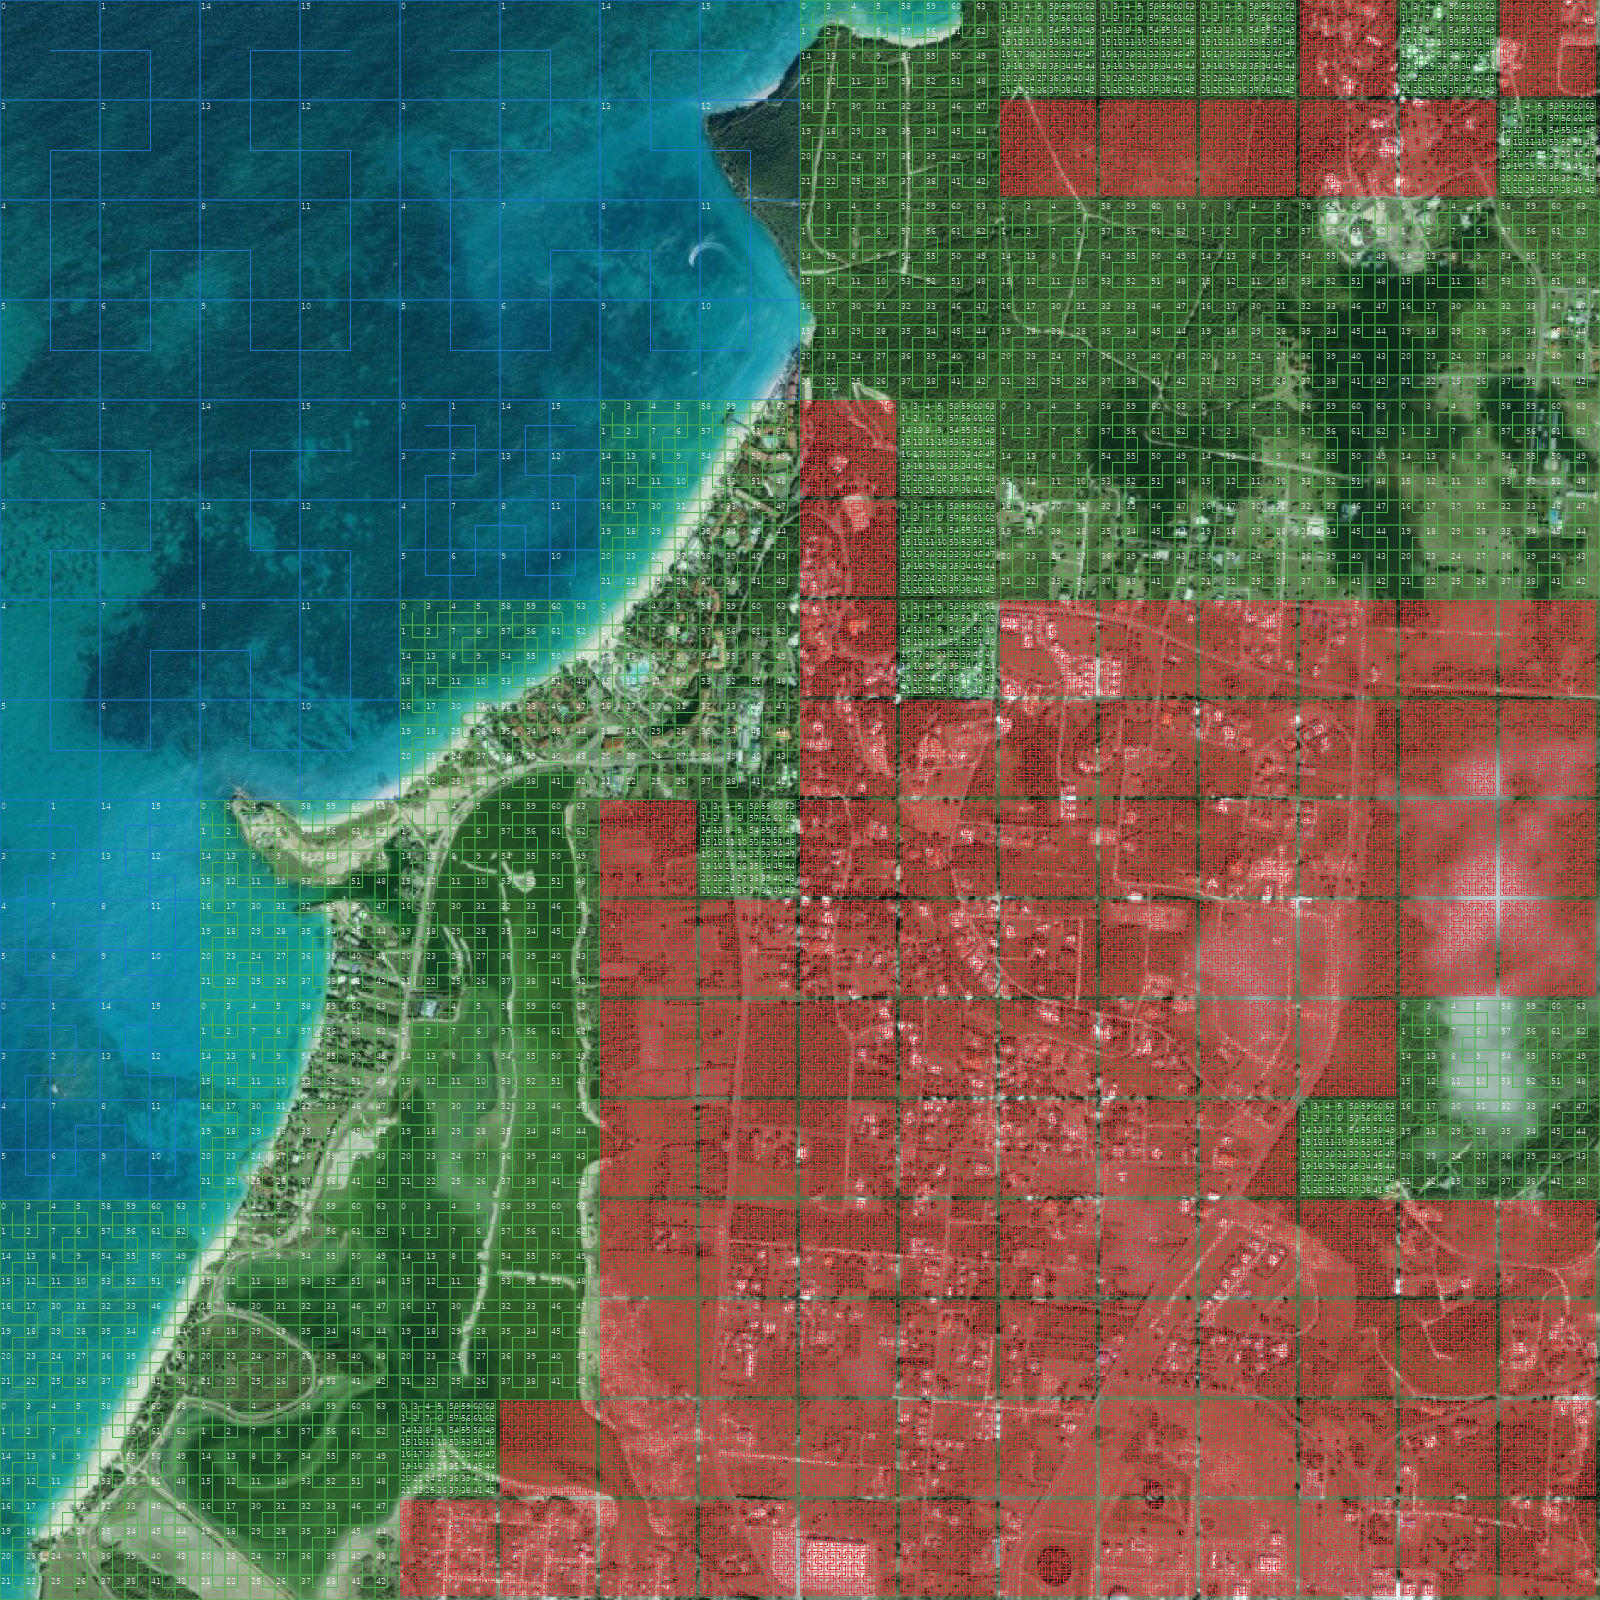
\includegraphics[width=0.8\textwidth]{images/adaptive_hilbert_index_vis.png}
    \caption{Adaptive Hilbert Indexing.}
\end{figure}

\subsection{Stage 3: Hybrid Tile Pyramid Construction}
To prevent visual artifacts, the builder aggressively crops the image bounding box to be an exact multiple of the 256px \texttt{TILE\_SIZE}, eliminating dead black spaces.

The pyramid is built dynamically:
\begin{itemize}
    \item \textbf{Fine Details (Zoom $\geq$ Threshold):} Directly rendered (cropped) from the source array.
    \item \textbf{Overviews (Zoom $<$ Threshold):} Uses a resampling algorithm, loading four $256\times256$ child tiles ($2\times2$ grid) into a $512\times512$ composite, and applying a high-quality \texttt{LANCZOS} downsample back to $256\times256$.
\end{itemize}

\begin{figure}[H]
    \centering
    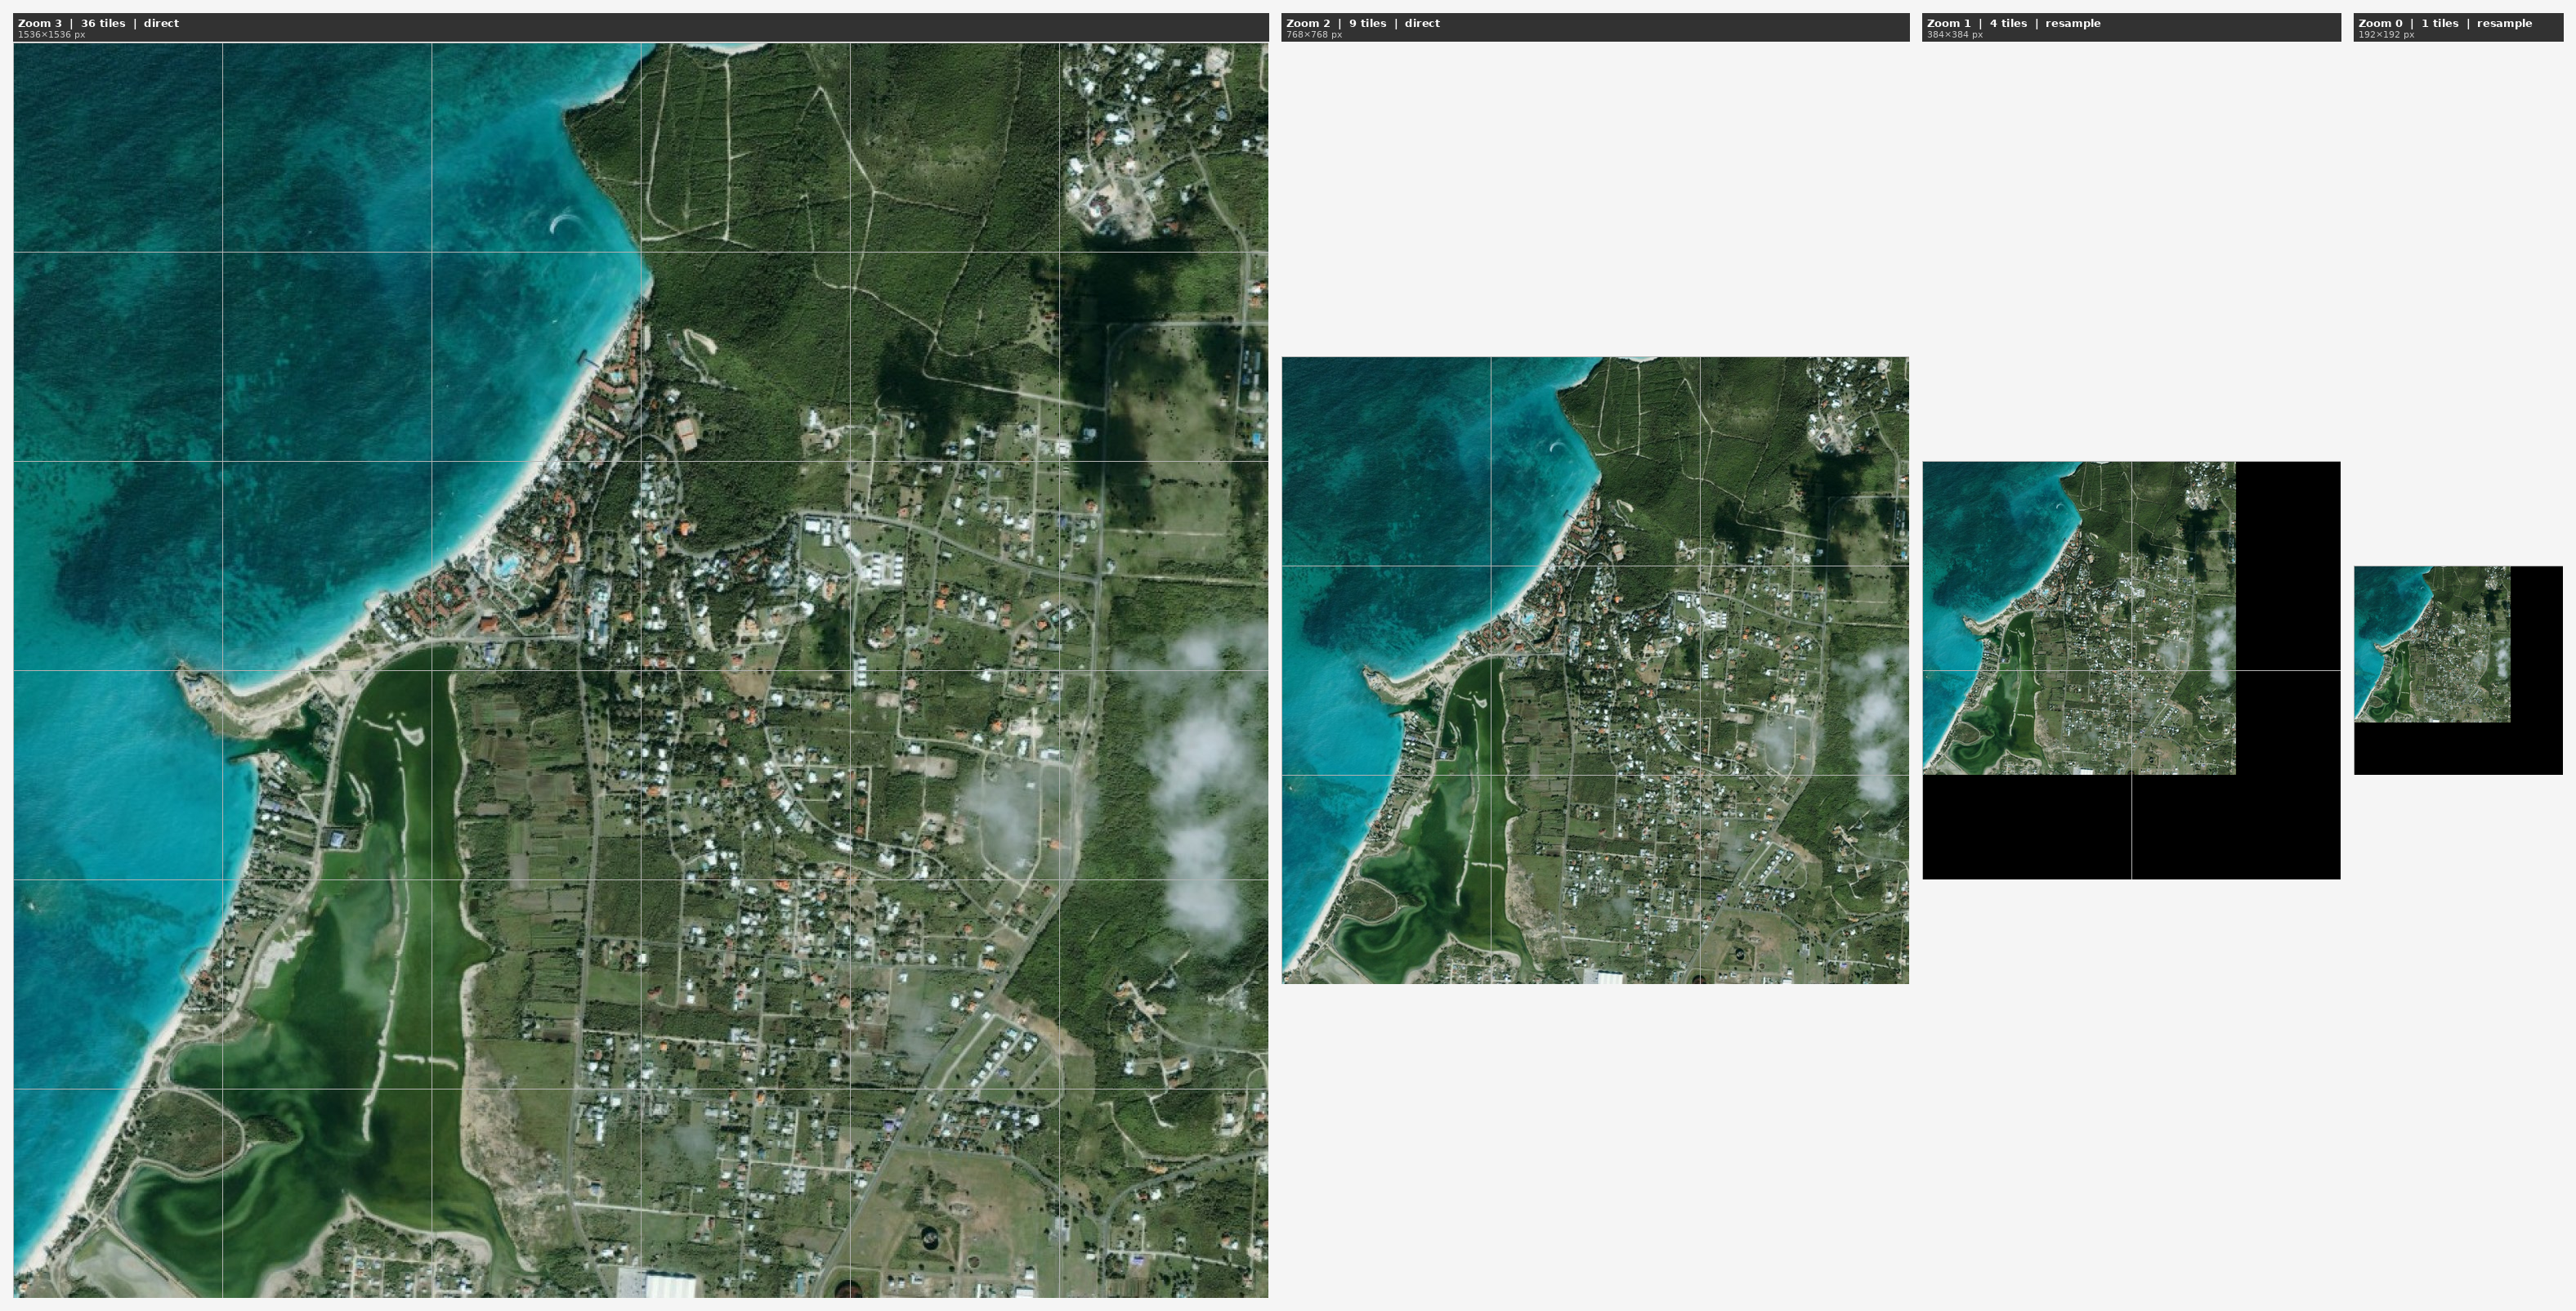
\includegraphics[width=0.8\textwidth]{images/pyramid_summary_visualization.png}
    \caption{Pyramid Generation Visualization.}
\end{figure}

\subsection{Stage 4: In-Memory Server Data Structures}
At server startup, \texttt{tile\_server.py} ingests the JSON mapping and populates highly optimized RAM structures to prevent disk I/O bottlenecks:
\begin{enumerate}
    \item \textbf{\texttt{INDEX}}: Flat array containing all tile metadata.
    \item \textbf{\texttt{BASE\_LOOKUP}}: Dictionary mapping \texttt{(base\_tx, base\_ty)} to its respective sub-tiles.
    \item \textbf{\texttt{BASE\_KEYS}}: Extracted array of just the sorted Hilbert integer codes corresponding to \texttt{BASE\_LOOKUP} to permit lightning-fast \texttt{bisect} searches.
    \item \textbf{\texttt{base\_rtree}}: A spatial R-Tree bounding-box index built strictly around the macroscopic quadtree base-tiles (not sub-tiles!).
    \item \textbf{\texttt{HILBERT\_CACHE}}: A precomputed lookup table storing all \texttt{xy\_to\_hilbert} spatial translations for Orders 2 through 7. This completely bypasses the mathematical Butz algorithm during real-time zoom queries.
\end{enumerate}

\subsection{Stage 5: The 4-Step Query Engine}
When a viewport query \texttt{(cx, cy, zoom)} is triggered, the \texttt{\_hilbert\_range\_scan} executes:
\begin{enumerate}
    \item \textbf{R-Tree Intersection $O(\log B + K_b)$:} The viewport bounding box intersects the \texttt{base\_rtree} to instantly prune distant quadtree leaves, returning only the candidate base tiles.
    \item \textbf{Local Cell Projection \& Cache Lookup:} For each candidate base tile, the viewport coordinates are mathematically mapped into the base tile's local sub-grid layout $(sx, sy)$. The code retrieves the precomputed Hilbert code from \texttt{HILBERT\_CACHE}.
    \item \textbf{Code Range Merging:} Overlapping, scattered cells are mathematically grouped into contiguous (start\_code, end\_code) bounding limits.
    \item \textbf{Local Array Bisect $O(\log N + K)$:} Binary search (\texttt{bisect\_left} and \texttt{bisect\_right}) jumps into the isolated \texttt{BASE\_KEYS} array of that specific base tile, slicing out the data. A final geometric confirmation drops edge false-positives.
\end{enumerate}

\section{Dynamic Visual Render Order (Zoom-based Recalculation)}
A crucial architectural distinction in the SAH system is the decoupling of the \textbf{Base Index Order} (used by the query engine) and the \textbf{Display Render Order} (used purely for visual context on the frontend).

\begin{enumerate}
    \item \textbf{Base Index Order (Fixed)}: Determined by the quadtree depth and semantic complexity at ingestion time. This controls exactly how many sub-cell records exist in the \texttt{BASE\_KEYS} arrays (e.g. 16 cells for Order 2). It \textit{never} changes.
    \item \textbf{Display Render Order (Dynamic)}: When the frontend zooms deeply into a collapsed tile, drawing a coarse $4\times4$ grid becomes visually unhelpful. Therefore, the visual Hilbert curve drawn on the React canvas is freshly recomputed in real-time based on zoom depth. As seen in \texttt{HilbertViewer.jsx}, the visual grid density scales dynamically when deeply zoomed.
\end{enumerate}

This means a water tile at zoom depth 3 will visually draw a highly dense curve on screen, providing rich spatial context to the user, while the underlying query engine remains blazing fast because it only bisects against the original 16 sub-cells. \textbf{The denser curve you see growing as you zoom is purely cosmetic and dynamically synthesized on the client.}

\begin{figure}[H]
    \centering
    \begin{minipage}{0.24\textwidth}
        \centering
        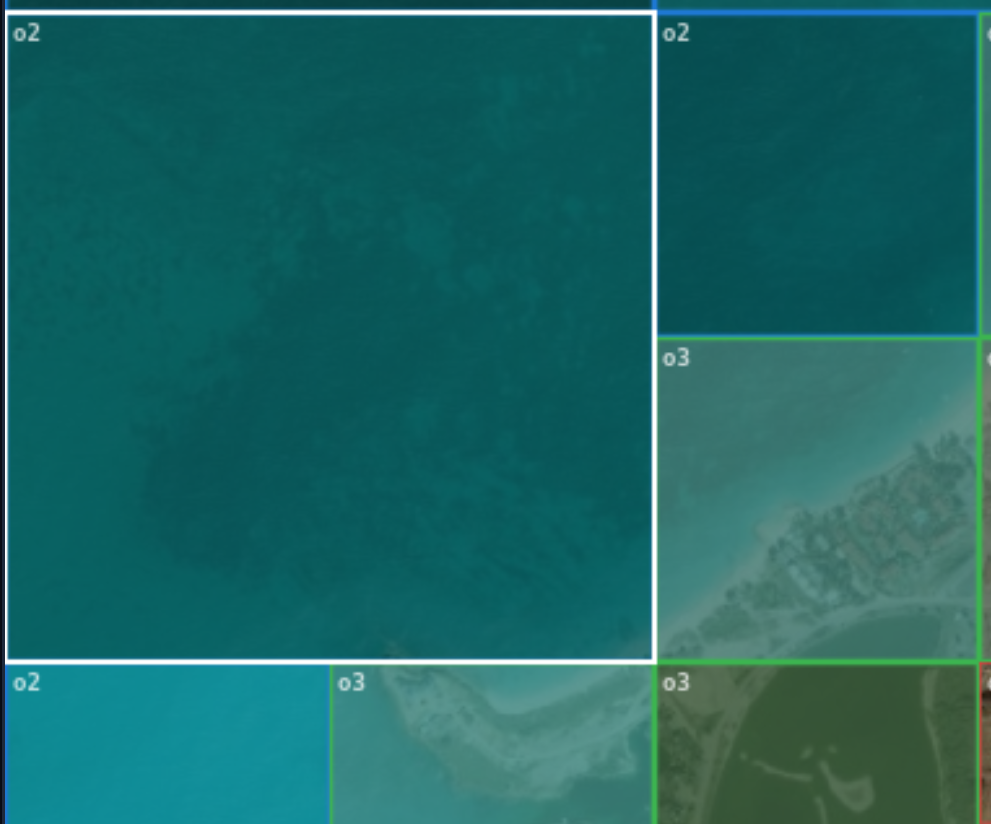
\includegraphics[width=\linewidth]{images/zoom0.png}
        \caption*{Zoom Level 0}
    \end{minipage}\hfill
    \begin{minipage}{0.24\textwidth}
        \centering
        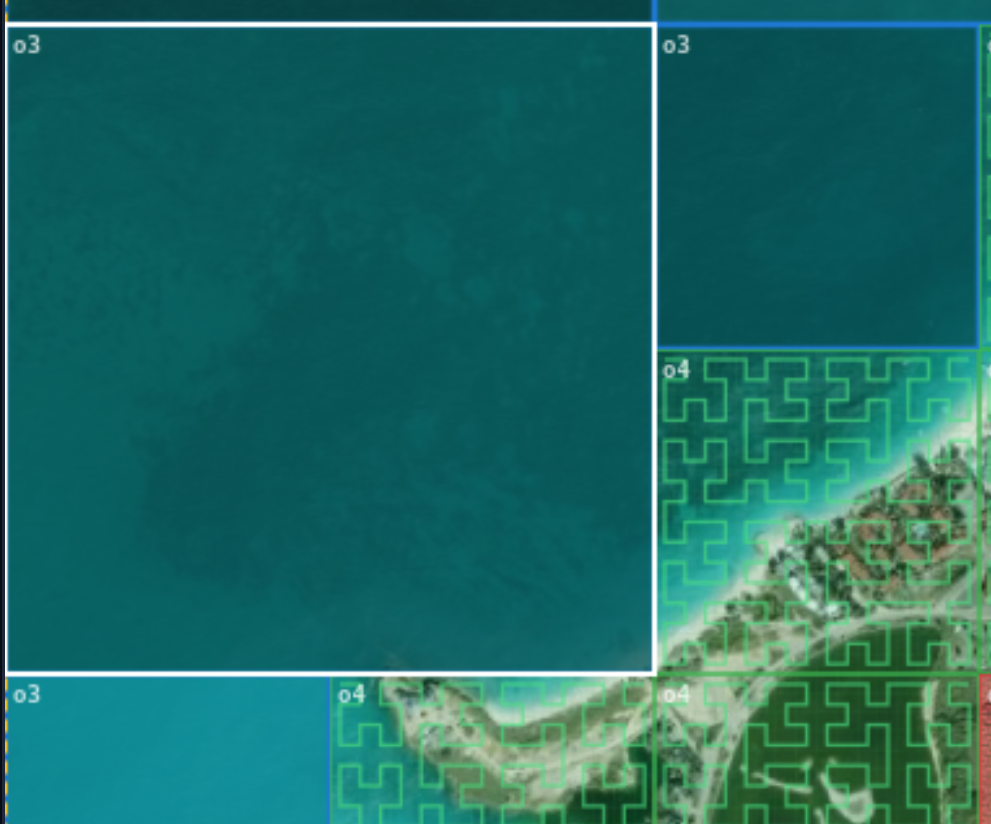
\includegraphics[width=\linewidth]{images/zoom1.png}
        \caption*{Zoom Level 1}
    \end{minipage}\hfill
    \begin{minipage}{0.24\textwidth}
        \centering
        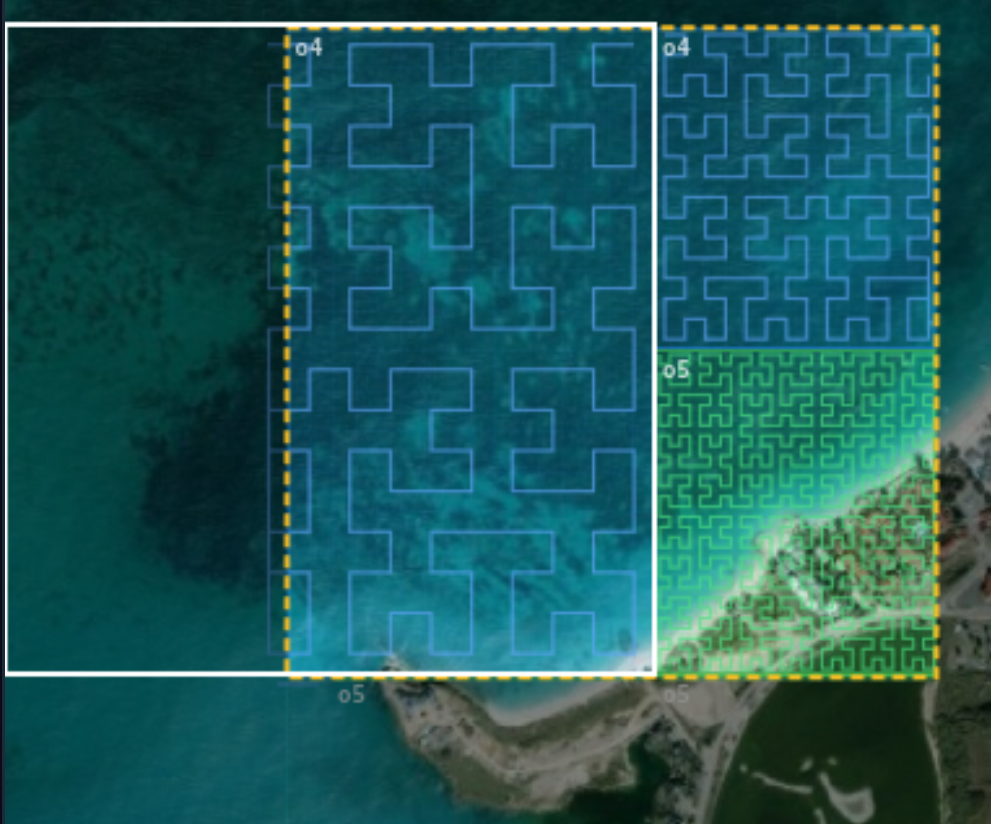
\includegraphics[width=\linewidth]{images/zoom2.png}
        \caption*{Zoom Level 2}
    \end{minipage}\hfill
    \begin{minipage}{0.24\textwidth}
        \centering
        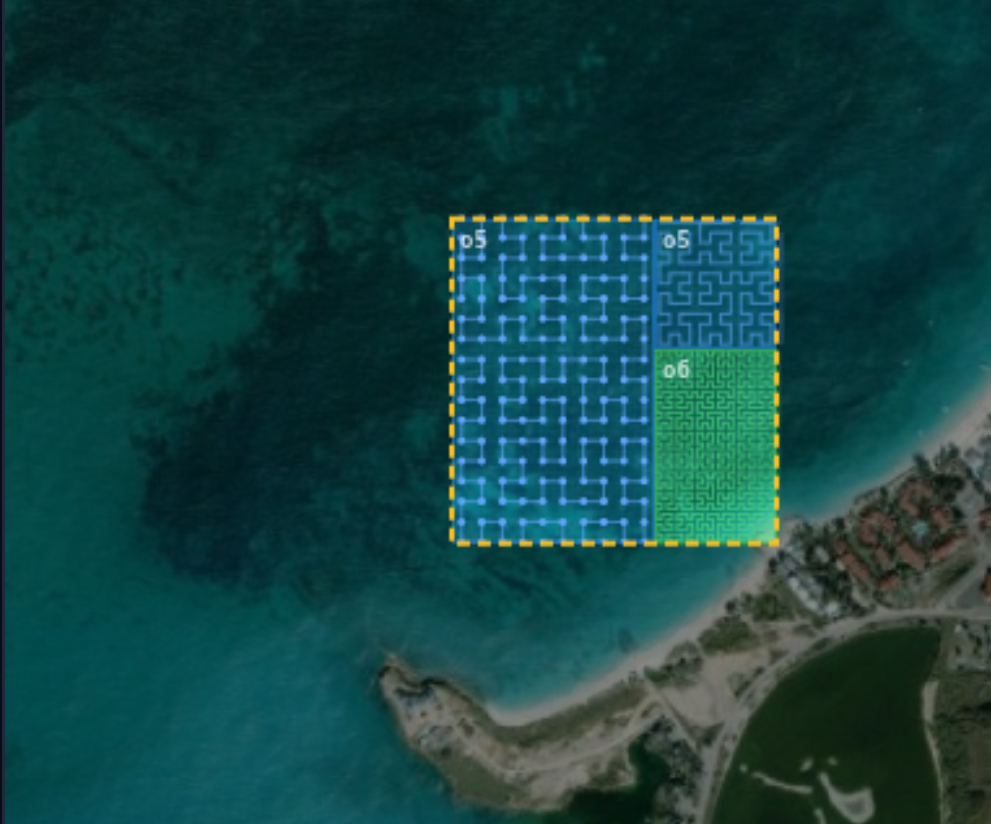
\includegraphics[width=\linewidth]{images/zoom3.png}
        \caption*{Zoom Level 3}
    \end{minipage}
    \caption{The visual Hilbert curve path is dynamically recomputed on the frontend canvas per zoom level, entirely independent of the rigid backend indexing.}
\end{figure}

\section{Algorithmic Complexity}
By utilizing \texttt{rtree\_mod} for macro-filtering and local array \texttt{bisect} for micro-filtering, SAH vastly outperforms legacy spatial databases:

\begin{table}[H]
    \centering
    \begin{tabularx}{\textwidth}{l X X}
        \toprule
        \textbf{Feature} & \textbf{Legacy Naive Scan} & \textbf{SAH Query Pipeline} \\
        \midrule
        \textbf{Grid Generation} & Uniform, symmetrical & Asymmetric, coastline-aware quadtree \\
        \textbf{Search Space} & Entire database (\texttt{INDEX}) & Localized strictly to \texttt{BASE\_KEYS} \\
        \textbf{Code Translation} & Calculated on the fly & Constant time via \texttt{HILBERT\_CACHE} \\
        \textbf{Spatial Check Time} & $O(N)$ & $O(\log B + \log N + K)$ \\
        \textbf{Off-screen Rejection} & Slow, linear check & Aggressive $\sim99\%$ permanent pruning \\
        \bottomrule
    \end{tabularx}
\end{table}

\noindent \textit{(B = Base quadtree tiles, N = Sub-tiles per base tile, K = Sub-tiles in viewport)}.

\section{Dual Render Output Environments}
The exact same \texttt{tile\_server.py} backend feeds multiple display contexts:

\subsection{Condition A — Standalone React Display}
A React canvas interacts directly with the API. At low zoom levels, regions designated as "collapsed" draw precomputed mean-color solid rectangles to aggressively conserve RAM. At high zoom, they unpack and fetch live PNGs from the tile store.

\begin{figure}[H]
    \centering
    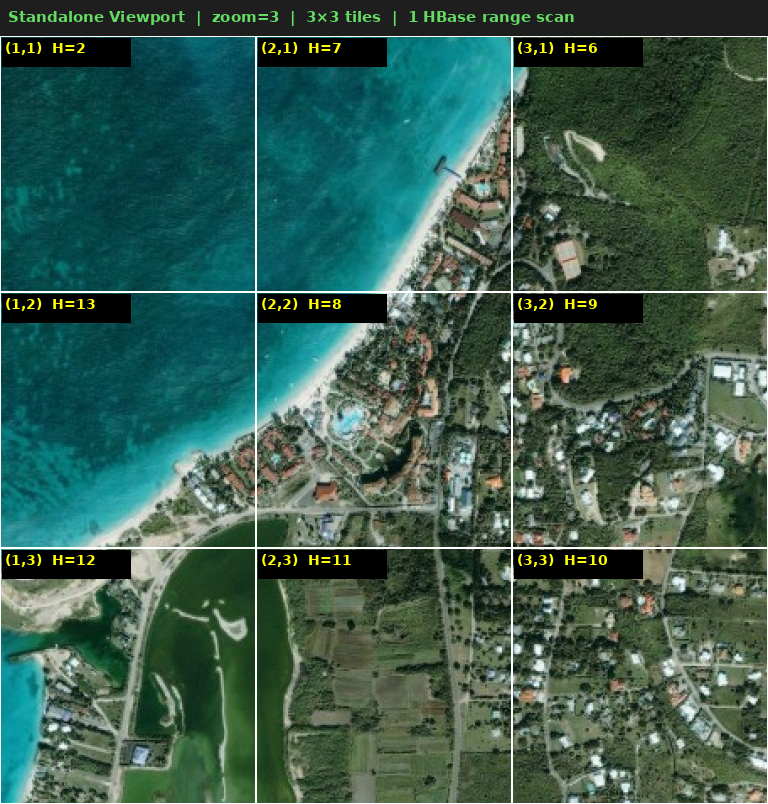
\includegraphics[width=0.8\textwidth]{images/integration_standalone_view.png}
    \caption{Standalone Display Output}
\end{figure}

\subsection{Condition B — Distributed SAGE2 Wall}
For multi-monitor interactive walls, \texttt{sage2\_display\_coordinator} clusters the Hilbert boundary space across physical UI panels. The identical query sequence is parallelized, fetching non-overlapping viewport intersections over WebSocket, stitching gigapixel frames inside 30fps rendering budgets.

\begin{figure}[H]
    \centering
    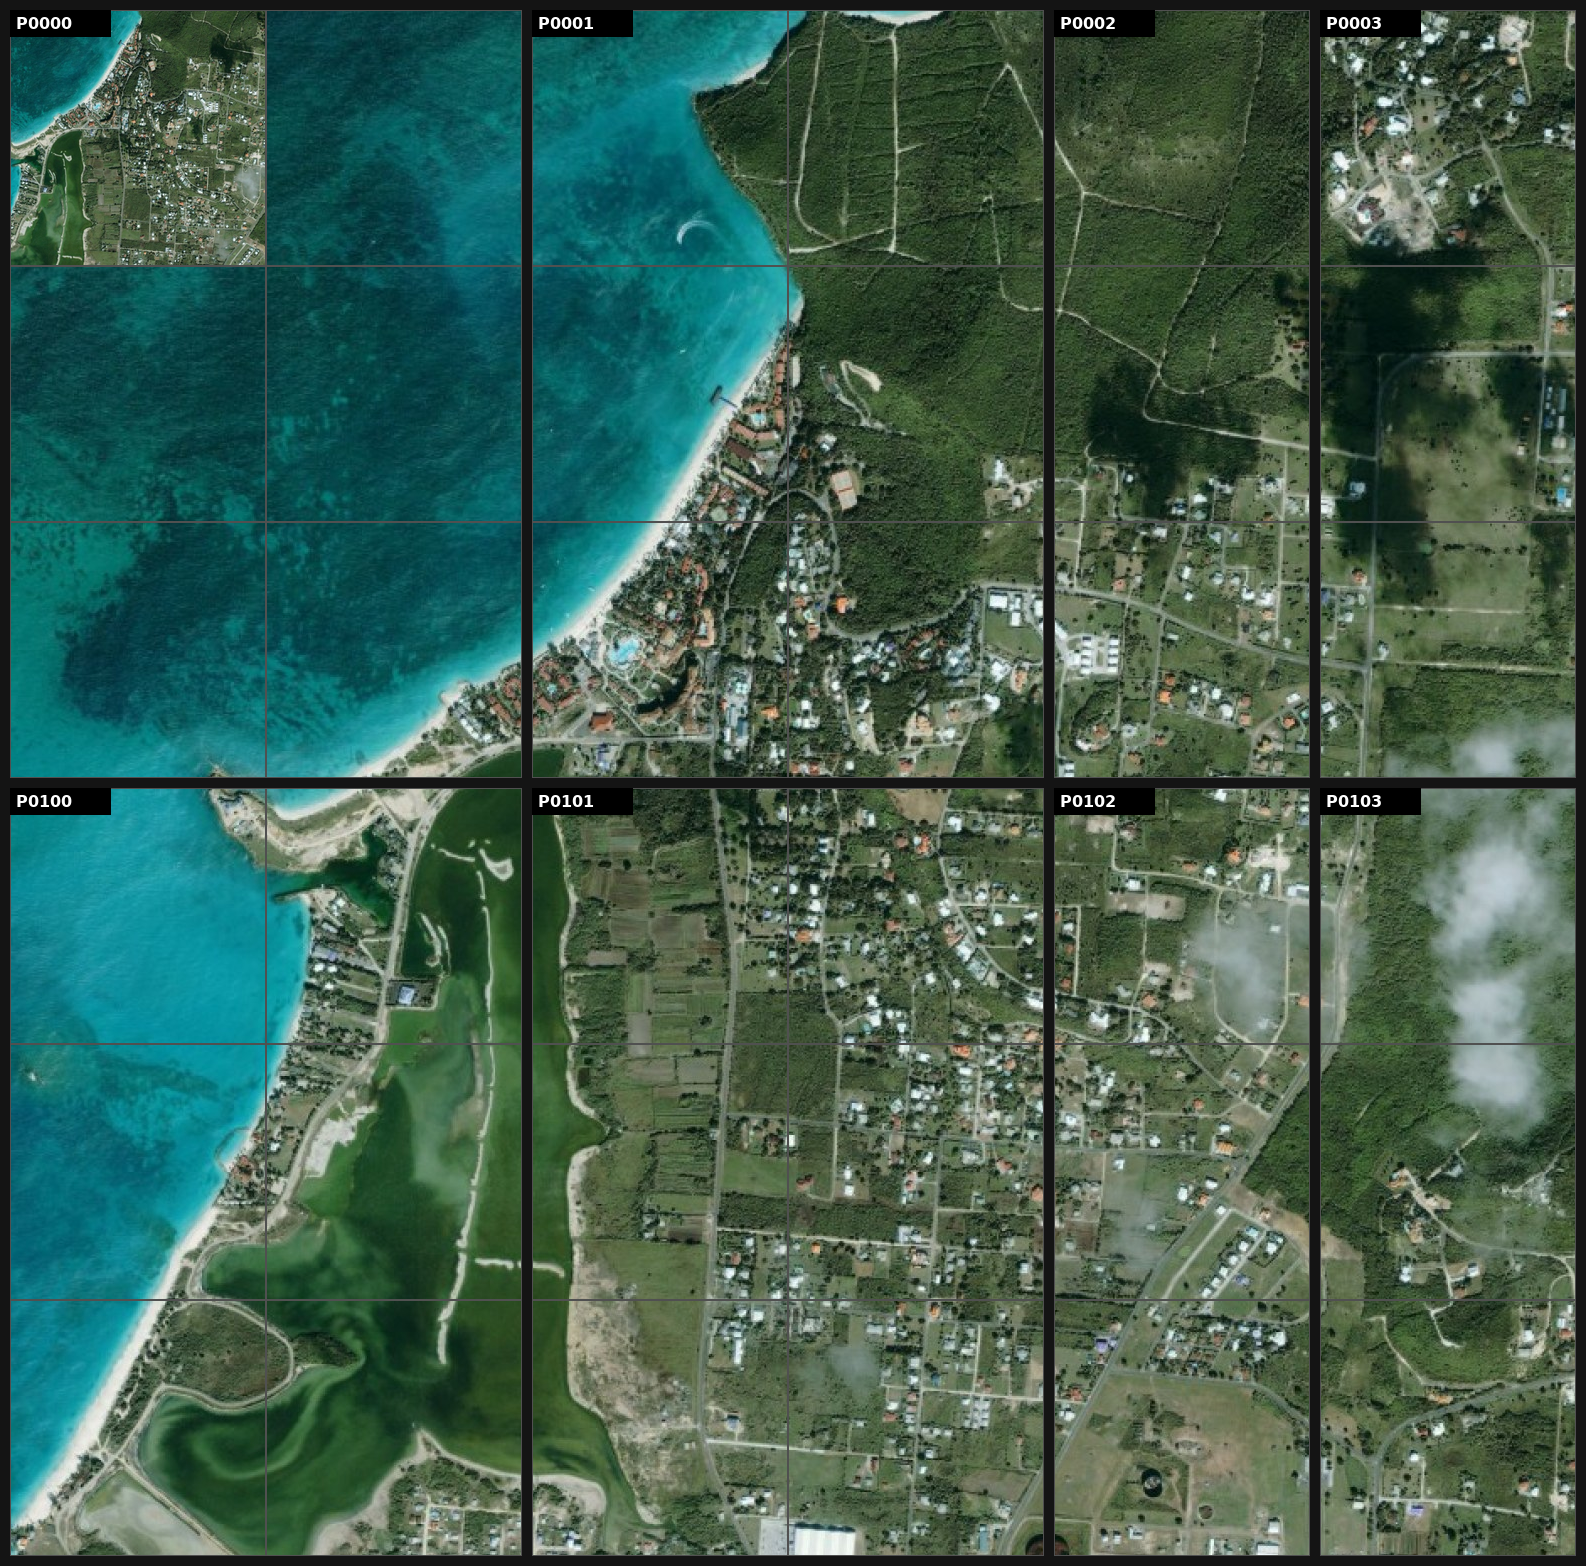
\includegraphics[width=0.8\textwidth]{images/integration_wall_view.png}
    \caption{Distributed Wall Display Output}
\end{figure}

\end{document}
